\documentclass[border=5mm]{standalone}
\usepackage{tikz}

\begin{document}
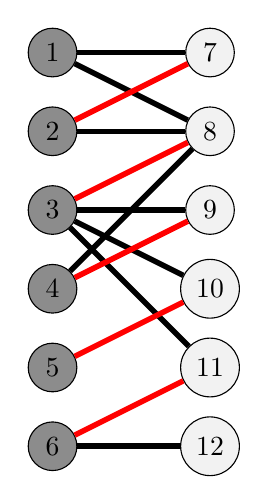
\begin{tikzpicture}[every tree node/.style={draw, circle, inner sep=2pt, text width=1.5em, align=center}]

    \node[draw, fill=gray!90, circle] (1) at (-1, -1) {1};
    \node[draw, fill=gray!90, circle] (2) at (-1, -2) {2};
    \node[draw, fill=gray!90, circle] (3) at (-1, -3) {3};
    \node[draw, fill=gray!90, circle] (4) at (-1, -4) {4};
    \node[draw, fill=gray!90, circle] (5) at (-1, -5) {5};
    \node[draw, fill=gray!90, circle] (6) at (-1, -6) {6};
    \node[draw, fill=gray!10, circle] (7) at (1, -1) {7};
    \node[draw, fill=gray!10, circle] (8) at (1, -2) {8};
    \node[draw, fill=gray!10, circle] (9) at (1, -3) {9};
    \node[draw, fill=gray!10, circle] (10) at (1, -4) {10};
    \node[draw, fill=gray!10, circle] (11) at (1, -5) {11};
    \node[draw, fill=gray!10, circle] (12) at (1, -6) {12};

    \draw[line width=2pt] (1) -- (7);
    \draw[line width=2pt] (1) -- (8);
    \draw[line width=2pt] (2) -- (8);
    \draw[line width=2pt] (3) -- (9);
    \draw[line width=2pt] (3) -- (10);
    \draw[line width=2pt] (3) -- (11);
    \draw[line width=2pt] (4) -- (8);
    \draw[line width=2pt] (6) -- (12);

    \draw[line width=2pt, color=red] (2) -- (7);
    \draw[line width=2pt, color=red] (3) -- (8);
    \draw[line width=2pt, color=red] (4) -- (9);
    \draw[line width=2pt, color=red] (5) -- (10);
    \draw[line width=2pt, color=red] (6) -- (11);



\end{tikzpicture}
\end{document}
